\documentclass[12pt]{article}
\usepackage[paper=letterpaper,margin=1.5cm]{geometry}
\usepackage{amsmath}
\usepackage{amssymb}
\usepackage{amsfonts}
\usepackage{mathtools}
%\usepackage[utf8]{inputenc}
%\usepackage{newtxtext, newtxmath}
\usepackage{lmodern}     % set math font to Latin modern math
\usepackage[T1]{fontenc}
\renewcommand\rmdefault{ptm}
%\usepackage{enumitem}
\usepackage[shortlabels]{enumitem}
\usepackage{titling}
\usepackage{graphicx}
\usepackage[colorlinks=true]{hyperref}
\usepackage{setspace}
\usepackage{subfigure} 
\usepackage{braket}
\usepackage{color}
\usepackage{tabularx}
\usepackage[table]{xcolor}
\usepackage{listings}
\usepackage{mathrsfs}
\usepackage{stackengine}
\usepackage{physics}
\usepackage{afterpage}
\usepackage{pdfpages}
\usepackage[export]{adjustbox}
\usepackage{biblatex}

\setstackEOL{\\}

\definecolor{dkgreen}{rgb}{0,0.6,0}
\definecolor{gray}{rgb}{0.5,0.5,0.5}
\definecolor{mauve}{rgb}{0.58,0,0.82}


\lstset{frame=tb,
  language=Python,
  aboveskip=3mm,
  belowskip=3mm,
  showstringspaces=false,
  columns=flexible,
  basicstyle={\small\ttfamily},
  numbers=none,
  numberstyle=\tiny\color{gray},
  keywordstyle=\color{blue},
  commentstyle=\color{dkgreen},
  stringstyle=\color{mauve},
  breaklines=true,
  breakatwhitespace=true,
  tabsize=3
}
\setlength{\droptitle}{-6em}

\makeatletter
% we use \prefix@<level> only if it is defined
\renewcommand{\@seccntformat}[1]{%
  \ifcsname prefix@#1\endcsname
    \csname prefix@#1\endcsname
  \else
    \csname the#1\endcsname\quad
  \fi}
% define \prefix@section
\newcommand\prefix@section{}
\newcommand{\prefix@subsection}{}
\newcommand{\prefix@subsubsection}{}
\renewcommand{\thesubsection}{\arabic{subsection}}
\makeatother
\DeclareMathOperator*{\argmin}{argmin}
\newcommand{\partbreak}{\begin{center}\rule{17.5cm}{2pt}\end{center}}
\newcommand{\alignbreak}{\begin{center}\rule{15cm}{1pt}\end{center}}
\newcommand{\tightalignbreak}{\vspace{-5mm}\alignbreak\vspace{-5mm}}
\newcommand{\hop}{\vspace{1mm}}
\newcommand{\jump}{\vspace{5mm}}
\newcommand{\R}{\mathbb{R}}
\newcommand{\C}{\mathbb{C}}
\newcommand{\N}{\mathbb{N}}
\newcommand{\G}{\mathbb{G}}
\renewcommand{\S}{\mathbb{S}}
\newcommand{\bt}{\textbf}
\newcommand{\xdot}{\dot{x}}
\renewcommand{\star}{^{*}}
\newcommand{\ydot}{\dot{y}}
\newcommand{\lm}{\mathrm{\lambda}}
\renewcommand{\th}{\theta}
\newcommand{\id}{\mathbb{I}}
\newcommand{\si}{\Sigma}
\newcommand{\Si}{\si}
\newcommand{\inv}{^{-1}}
\newcommand{\T}{^\intercal}
\renewcommand{\tr}{\text{tr}}
\newcommand{\ep}{\varepsilon}
\newcommand{\ph}{\varphi}
%\renewcomand{\norm}[1]{\left\lVert#1\right\rVert}
\definecolor{cit}{rgb}{0.05,0.2,0.45}
\addtolength{\jot}{1em}
\newcommand{\solution}[1]{

\noindent{\color{cit}\textbf{Solution:} #1}}

\newcounter{tmpctr}
\newcommand\fancyRoman[1]{%
  \setcounter{tmpctr}{#1}%
  \setbox0=\hbox{\kern0.3pt\textsf{\Roman{tmpctr}}}%
  \setstackgap{S}{-.9pt}%
  \Shortstack{\rule{\dimexpr\wd0+.1ex}{.9pt}\\\copy0\\
              \rule{\dimexpr\wd0+.1ex}{.9pt}}%
}

\newcommand{\Id}{\fancyRoman{2}}

% Enter the specific assignment number and topic of that assignment below, and replace "Your Name" with your actual name.
\title{Class 31210: Cheat Sheet}
\author{Caleb Derrickson}
\date{March 4, 2024}

\begin{document}
\onehalfspacing
\maketitle
\allowdisplaybreaks
\tableofcontents

\newpage

\section{Chapter 5}
\boxedquote{Hahn-Banach Theorem}{
    If $Y$ is a linear subspace of a normed linear space $X$ and $\psi: Y \rightarrow \mathbb{R}$ is a bounded linear functional on $Y$ with $\|\psi\| = M$, then there is a bounded linear functional $\varphi : X \rightarrow \mathbb{R}$ such that $\varphi$ restricted to $Y$ is equal to $\psi$ and $\|\varphi\| = M$.
}

To show that an operator $K: X \to Y$ is compact, we need to show that for any bounded subset $B \subset X$, that $K(B)$ is precompact. That means that its closure is compact. 

\boxedquote{Arzel\'a - Ascoli}{Let $K$ be a compact metric space. A subset of $C(K)$ is compact if and only if it is closed, bounded, and equicontinuous.}

\mquote{Equicontinuity}{Let $\scF$ be a family of functions from a \textbf{metric space} $(X, d)$ to a metric space $(Y, d)$. The family $\scF$ is \textit{equicontinuous} if for every $x \in X$ and $\ep > 0$ there exists a $\delta > 0$ such that $d(x, y) < \delta \implies d(f(x), f(y)) < \ep$ for all $f \in \scF$.}

The important thing about this definition is that $\delta$ does not depend on $f$, it could depend on $x$, though.

\boxedquote{Convergence}{
\begin{enumerate}
    \item \underline{Uniform convergence}: For a sequence (anything, linear operator, operator, sequence, ...) $x_n$ which converges to $x$, we have that $\lim_{n \to \infty} \norm{x_n - x} = 0$.

    \item \underline{Strong convergence}: Same as uniform convergence. For functions, it is pointwise on sup norm. 

    \item \underline{Weak convergence}: 
    \begin{itemize}
        \item \textbf{For Banach Spaces}: If $X$ is a Banach space, and $X\star$ is its dual, then $x_n$ converges weakly to $x$, denoted by $x_n \rightharpoonup x$ as $n \to \infty$ if $\ph (x_n) \to \ph(x)$ as $n \to \infty$ for every bounded linear functional $\ph \in X\star$.
        \item \textbf{For Hilbert Spaces}: By the Reisz Representation Theorem, we can relate any bounded linear functional $\ph \in \scH \star$ to an inner product with a \textit{unique} $y \in \scH$ such that $\braket{x_n}{y} \rightarrow \braket{x}{y}$ as $n \to \infty$. 
    \end{itemize}
    
    \item \underline{Weak$*$ - convergence}: This only relates to Banach spaces, since weak$*$ convergence in Hilbert spaces is the same as weak convergence. For $X$ Banach, and $X\star$ its dual, then for a sequence $\ph_n$, $\ph_n \overset{*}{\rightharpoonup} \ph$ if $\ph_n(x) \to \ph(x)$ for any $x \in X$.
\end{enumerate}
}

\newpage
\section{Chapter 12}
\boxedquote{Dominate Convergence Theorem}{Suppose that $(f_n)$ is a sequence of square integrable functions, $f_n : X \to \overline{\R}$, on a measure space $(X, A, \mu)$ that converges pointwise to a limiting function $f: X \to \overline{\R}$. If there is an integrable function $g : X \to [0, \infty]$ such that 
\[|f_n(x)| \leq g(x) \quad \text{for all $x \in X$ and $n \in \N$},\]
then $f$ is integrable and 
\[\lim_{n \to \infty} \int f_n \ d\mu = \int f \ d\mu.\]}

\boxedquote{Corollary 12.36}{Suppose that $(X, A , \mu)$ is a complete measure space, $I \subset \R$ is an open interval, and $f : X \times I \into \overline{\R}$ is a measurable function such that:
        \begin{itemize}
            \item $f(\cdot, t)$ is integrable on $X$ for each $t \in I$;
            \item $f(x, \cdot)$ is differentiable in $I$ for each $x \in X \setminus N$, where $\mu(N) = 0$;
            \item there is an integrable function $g: X \into [0, \infty]$ such that 
            \[ \left| \frac{\partial f}{\partial t}(x, t) \right| \leq g(x) \quad \text{a.e. in $X$ for every $t \in I$.}\]
            Then
            \[\ph (t) = \int_X f(x, t) \ d\mu(x)\]
            is a differentiable function of $t$ in $I$, and 
            \[\frac{d\ph}{dt} (t) = \int_X \frac{\partial f}{\partial t}(x, t) \ d\mu(x).\]
            \end{itemize}
    }

\newpage
\section{Chapter 6}
\begin{itemize}
    \item Hilbert spaces are COMPLETE inner product spaces.

\item The space $L^p([a, b])$, given as the set of square integrable functions, is a Hilbert space ONLY WHEN $p = 2$. The rest are banach spaces. The inner product is given as
\[\braket{f}{g} = \int_I \overline{f(x)} g(x) \ dx\]
and the norm is given by 
\[\norm{f}^2 = \int_I |f(x)|^2 \ dx\]

\item $\ell^2(\Z \text{ or } \N)$ is defined as square summable sequences. 

\boxedquote{Parallelogram Law}{A normed linear space $X$ is an inner product space with a norm derived from the inner product iff
\[\norm{x + y}^2 + \norm{x - y}^2 = 2\norm{x}^2 + 2\norm{y}^2 \quad \text{for all $x, y \in X$}.\]}

If a norm satisfies the parallelogram law, then the inner product defined below defines an inner product on $X$. 
\[\braket{x}{y} = \frac{1}{4}\left\{ \norm{x + y}^2 - \norm{x - y}^2 - i\norm{x + iy}^2 + i\norm{x - iy}^2\right\}\]

\item Inner product is a continuous map from $X \times X \to \C$.

\item The orthogonal complement of a SUBSET of a Hilbert space is a CLOSED linear space. 

\boxedquote{Projection}{Let $\scM$ be a closed linear subspace of a Hilbert space $\scH$.
\begin{itemize}
    \item[a)] For each $x \in \scH$, there is a unique closest point $y \in \scM$ such that 
    \[\norm{x - y} = \min_{z \in \scM}\norm{x - z}\]
    \item[b)] The point $y \in \scM$ closest to $x \in \scH$ is the unique element of $\scM$ with the property that $(x - y)\perp \scM$.
\end{itemize}
}

\mquote{Orthogonal Direct Sum}{If $\scM$ and $\scN$ are closed linear subspaces of a Hilbert spaces, then 
\[\scM \oplus \scN = \{y + z : y \in \scM \text{ and } z \in \scN\}\]}

\item If $\scM$ is a closed subspace of $\scH$, then $\scH = \scM \oplus \scM^\perp$.

\item EVERY HILBERT SPACE HAS AN ORTHONORMAL BASIS

\boxedquote{Bessel's Inequality}{Let $U = \{u_\alpha : \alpha \in I\}$ be an orthonormal SET in a Hilbert space $\scH$ and $x \in \scH$. Then:
\begin{enumerate}
    \item[a)] $\norm{x}^2 \geq \sum_{\alpha \in I}|\braket{u_\alpha}{x}|^2$
    \item[b)] $x_U = \sum_{\alpha \in I} \braket{u_\alpha}{x}u_\alpha$ is a convergent sum
    \item[c)] $x - x_U \in U^\perp$
\end{enumerate}
}

\boxedquote{Parseval's Identity}{If $U = \{u_\alpha : \alpha \in I\}$ is an orthonormal subset of a Hilbet space $\scH$, then the following are equivalent:
\begin{itemize}
    \item[a)] $\braket{u_\alpha}{x} = 0$ for all $\alpha \in I$ implies $x = 0$.
    \item[b)] $x = \sum_{\alpha \in I} \braket{u_\alpha}{x}u_\alpha$ for all $x \in \scH$
    \item[c)] $\norm{x}^2 = \sum_{\alpha \in I} |\braket{u_\alpha}{x}|^2$ for all $x \in \scH$
\end{itemize}
}

\item An Orthonormal set of a Hilbert space is complete if it satisfies Parseval's Identity. A complete orthonormal subset of $\scH$ is called the orthonormal basis of $\scH$.

\item Any subspace of a linear space is closed in finite dimensions.

\subsection{Hermite Polynomials}
This will relate to solving Problem 6.14. They are given by
\[H_n(x) = (-1)^n e^{x^2} \frac{d^n}{dx^n}\left(e^{-x^2}\right)\]
To show that the functions 
\[\ph_n(x) = e^{-x^2/x}H_n(x)\]
form an orthogonal set in $L^2(\R)$, we just need to show that $e^{-x^2/2}x^m$ is orthogonal to $\ph_n(x)$, for $n > m$. This is sufficient since polynomials of degree $m < n$ are immediately orthogonal to $\ph_n(x)$ in the $L^2(\R)$ inner product. Next, to show that $\ph_n$ is an eigenfunction of the linear operator 
\[H = -\frac{d^2}{dx^2} + x^2\]
with eigenvalue $\lm_n = 2n+1$, we should break this into two operators
\[A = \frac{d}{dx} + x, \quad A\star = -\frac{d}{dx} + x\]
and show that $AA\star - 1 = H$. Investigate the action both operators have on $\ph_n$. To simplify things, we can assume (or prove, depending on time) that 
\[\frac{dH_n}{dx} = 2nH_{n-1} = -H_{n+1} + 2xH_n\]

\end{itemize}

\newpage
\section{Chapter 7}
\begin{itemize}
    \item Fourier orthonormal basis: 
    \[e_n(x) = \frac{1}{\sqrt{2\pi}}e^{inx}\]
    \item Trigonometric polynomials are dense in $L^2(\scT)$ 
    \item Convolution of two continuous functions:
    \[(f\ast g)(x) = \int_\scT f(x - y) g(y) \ dy = \int_\scT f(y)g(x - y) \ dy\]
    \mquote{Approximate Identity}{A family of functions $\{\ph_n \in C(\scT) : n \in \N\}$ is an approximate identity if
    \begin{enumerate}
        \item[a)] $\ph_n(x) \geq 0$
        \item[b)] $\int_\scT \ph_n(x) \ dx = 1 \quad \text{for every $n \in \N$}$
        \item[c)] $\lim_{n \to \infty}\int_{\delta \leq |x| \leq \pi} \ph_n(x) \ dx = 0$ for every $\delta > 0$ 
    \end{enumerate}
    }

\boxedquote{Thm 7.2}{ If $\{\ph_n\in C(\scT) : n \in \N$ is an approximate identity and $f \in C(\scT)$, then $\ph_n \ast f$ converges UNIFORMLY to $f$ as $n \to \infty$.}

\boxedquote{Thm 7.3}{The trigonometric polynomials are dense in $C(\scT)$ with respect to the uniform norm.}

\item Fourier coefficients 
\[\hat{f} = \frac{1}{\sqrt{2\pi}}\int_\scT f(x) e^{-inx} \ dx\]

\item Fourier Expansion of $f \in L^2(\scT)$:
\begin{align*}
    &f(x) = \frac{1}{2}a_0 + \sum_{n = 1}^\infty \{ a_n \cos(nx) + b_n\sin(nx)\},\\
    &a_0 = \frac{1}{\pi}\int_{\scT} f(x) \ dx, \quad a_n = \frac{1}{\pi}\int_\scT f(x) \cos(nx) \ dx, \quad b_n = \frac{1}{\pi} \int_\scT f(x)\sin(nx) \ dx 
\end{align*}

\newpage
\subsection{Dirichlet kernel}
Both this subsection and the next will dedicated to problem 7.2, where we analyze the Dirichlet and Fej\'er kernel. The Dirichlet kernel can be written equivalently as
\[D_N = \frac{1}{2\pi}\frac{\sin[(N + 1/2)x]}{\sin(x/2)} = \frac{1}{2\pi}\sum_{n = -N}^Ne^{inx}\]
The latter will (probably) need to be proven, where we will get the first definition. The proof is 
 \[\frac{\sin [(n + 1/2)x]}{\sin(x/2)} = \frac{-2i\sin [(n + 1/2)x]}{-2i\sin(x/2)} = \frac{e^{-(n+1/2)ix} - e^{(n+1/2)ix}}{e^{-ix/2} - e^{ix/2}} = \sum_{k = -n}^n e^{ikx}\]
    The geometric series is used, where we extended to negative terms via
    \[\sum_{k = -n}^n r^k = r^{-n}\left[ \frac{1 - r^{2n+1}}{1-r}\right].\]

\subsection{Fej\'er Kernel}
The Fej\'er kernel is given as 
\[F_N(x) = \frac{1}{2\pi(N + 1)}\left(\frac{\sin[(N+1)x/2]}{\sin(x/2)}\right)^2\]
A better form, which we will likely need to prove, is given in terms of the Dirichlet kernel as 
\[F_N(x) = \frac{1}{N+1}\sum_{k = 0}^N D_k(x)\]
This is proven by 
\tightalignbreak
    \begin{align*}
        &F_N(x) = \frac{1}{N+1}\left(\frac{\sin\left[ (N+1)x/2\right]}{\sin(x/2)}\right)^2 &\text{(Given.)}\\
        &= \frac{1}{N+1}\frac{1}{\sin^2(x/2)}\left(\sin\left[ (N+1)x/2\right]\right)^2 &\text{(Rearranging.)}\\
        &= \frac{1}{N+1}\frac{1}{\sin^2(x/2)}\frac{1 - \cos \left[ (N+1)x\right]}{2} &\text{(Trig identity.)}\\
        &= \frac{1}{N+1}\frac{1}{2\sin^2(x/2)}\sum_{k = 0}^N \left[ \cos(kx) - \cos((k+1)x)\right] &\text{(Reinterpretation.)}\\
        &= \frac{1}{N+1}\frac{1}{\sin^2(x/2)}\sum_{k = 0}^N \left[ \sin((k+1/2)x) \sin(x/2)\right] &\text{(Trig identity.)}\\
        &= \frac{1}{N+1}\frac{1}{\sin(x/2)}\sum_{k = 0}^N \left[ \sin((k+1/2)x) \right] &\text{(Simplifying.)}\\
        &= \frac{1}{N+1}\sum_{k = 0}^N \frac{\left[ \sin((k+1/2)x) \right]}{\sin(x/2)} &\text{(Rearranging.)}\\
        &= \frac{1}{N+1}\sum_{k = 0}^N D_k(x) &\text{(Given.)} 
    \end{align*}
    \vspace{-12mm}\alignbreak

    \item THE DIRICHLET KERNEL IS NOT AN APPROXIMATE IDENTITY - IT FAILS TO BE STRICTLY POSITIVE. The Fej\'er kernel can be proven to be an approximate identity. 
\end{itemize}

\newpage
\section{Chapter 8}
\begin{itemize}
\item If $X$ is a linear space, then we define the projection $P: X \to X$ onto $M$ along $N$ by $Px = y$, where $x = y + z, \ y \in M, \ z \in N$. $\range(P) = M, \ \ker(P) = N$.
\boxedquote{Theorem 8.2}{Let $X$ be a linear space
\begin{itemize}
    \item[a)] If $P: X \to X$ is a projection, then $X = \range(P) \oplus \ker(P)$. 
    \item[b)] If $X = M \oplus N$, where $M$ and $N$ are linear subspaces of $X$, then there is a projection $P: X \to X$ with $\range(P) = M, \ \ker(P) = N$.
\end{itemize}
}

\item An ORTHOGONAL PROJECTION on a Hilbert Space $\scH$ is a linear map $P: \scH \to \scH$ that satisfies 
\[P^2 = P, \quad \braket{Px}{y} = \braket{x}{Py}\quad \text{for all } x, y \in \scH.\]

\item Nonzero Orthogonal projections have norm 1.
\item Orthogonal projections are by definition self-adjoint 

\boxedquote{Theorem 8.5}{Let $\scH$ be a Hilbert space. 
\begin{enumerate}
    \item[a)] If $P$ is an orthogonal projection on $\scH$, then $\range(P)$ is closed, and 
    \[\scH = \range(P) \oplus\ker(P)\]
    is the orthogonal direct sum of $\range(P)$ and $\ker(P)$. 
    \item[b)] If $\scM$ is a closed subspace of $\scH$, then there is an orthogonal projection $P$ on $\scH$ with $\range(P) = \scM$ and $\ker(P) = \scM^\perp$.
\end{enumerate}

}
\boxedquote{Riesz Representation}{If $\ph$ is a bounded linear functional on a Hilbert space $\scH$, then there is a unique vector $y \in \scH$ such that 
\[\ph(x) = \braket{y}{x} \quad \text{for all } x \in \scH\]
}

\item If $y \in \scH$, then $\ph_y(x) = \braket{y}{x}$ is a bounded linear functional on $\scH$ with $\norm{\ph_y} = \norm{y}.$

\item The Adjoint of a linear operator is unique and is a bounded linear operator. Note:
\[\braket{x}{Ay} = \braket{A\star x}{y} \quad \text{for all } x, y \in \scH\]

\newpage
\boxedquote{Theorem 8.17}{If $A: \scH \to \scH$ is a bounded linear operator, then 
\[\overline{\range(A)} = (\ker(A\star))^\perp, \quad \ker(A) = (\range(A\star))^\perp\]
}

\boxedquote{Lemma 8.26}{If $A$ is a bounded self-adjoint operator on a Hilbert space $\scH$, then 
\[\norm{A} = \sup_{\norm{x} = 1}|\braket{x}{Ax}| \]
}

\mquote{Corollary}{If $A$ is a bounded operator on a Hilbert space, then $\norm{A\star A} = \norm{A}^2$. If $A$ is self-adjoint, then $\norm{A^2} = \norm{A}^2$.}

\boxedquote{Uniform Boundedness}{
    Suppose that 
    \[\{\ph_n: X \to \C \ |\  n \in \N\}\]
    is a set of linear functionals on a Banach space $X$ such that the set of complex numbers $\{\ph_n(x) : n \in \N\}$ is bounded for each $x \in X$. Then $\{\norm{\ph_n} : n \in \N\}$ is bounded.
}

\mquote{Theorem 8.40}{Suppose that $x_n$ is a sequence in a Hilbert space $\scH$ and $D$ is a dense subset of $\scH$. Then $x_n$ converges weakly to $x$ if and only if:
\begin{itemize}
    \item[a)] $\norm{x_n} \leq M$ for some constant $M$
    \item[b)] $\braket{x_n}{y} \to \braket{x}{y}$ as $n \to \infty$ for all $y \in D$.
\end{itemize}
}

\boxedquote{Banach-Alaoglu}{The closed unit ball of a Hilbert space is weakly compact. For Banach spaces, the closed unit ball is weak-$\ast$ compact.}
\end{itemize}


\newpage
\section{Chapter 9}
\begin{itemize}
    \item The resolvent set of a bounded linear operator A, denoted by $\rho(A)$ is the set of complex numbers such that $(A - \lm\id)$ is bijective. 

    \item The spectrum, enote ad $\sigma(A)$ is the complement of the resolvent set in $\C$, so that $(A - \lm\id)$ is not bijective. We break into cases on how its not bijective.

    \begin{enumerate}
        \item If $\lm \in \sigma(A)$ makes it such that $(A - \lm\id)$ is not injective, then $\lm$ is in the \textbf{point spectrum} of A.
        \item If $\lm\in \sigma(A)$ makes it such that $(A - \lm\id)$ is injective, but not surjective, \textbf{and} $\range(A - \lm\id)$ is dense in $\scH$, then $\lm$ is in the \textbf{continuous spectrum} of $A$.
        \item If $\lm\in \sigma(A)$ makes it such that $(A - \lm\id)$ is injective, but not surjective, \textbf{and} $\range(A - \lm\id)$ is not dense in $\scH$, then $\lm$ is in the \textbf{residual spectrum} of $A$.
    \end{enumerate}
    \begin{figure}[!h]
        \centering
        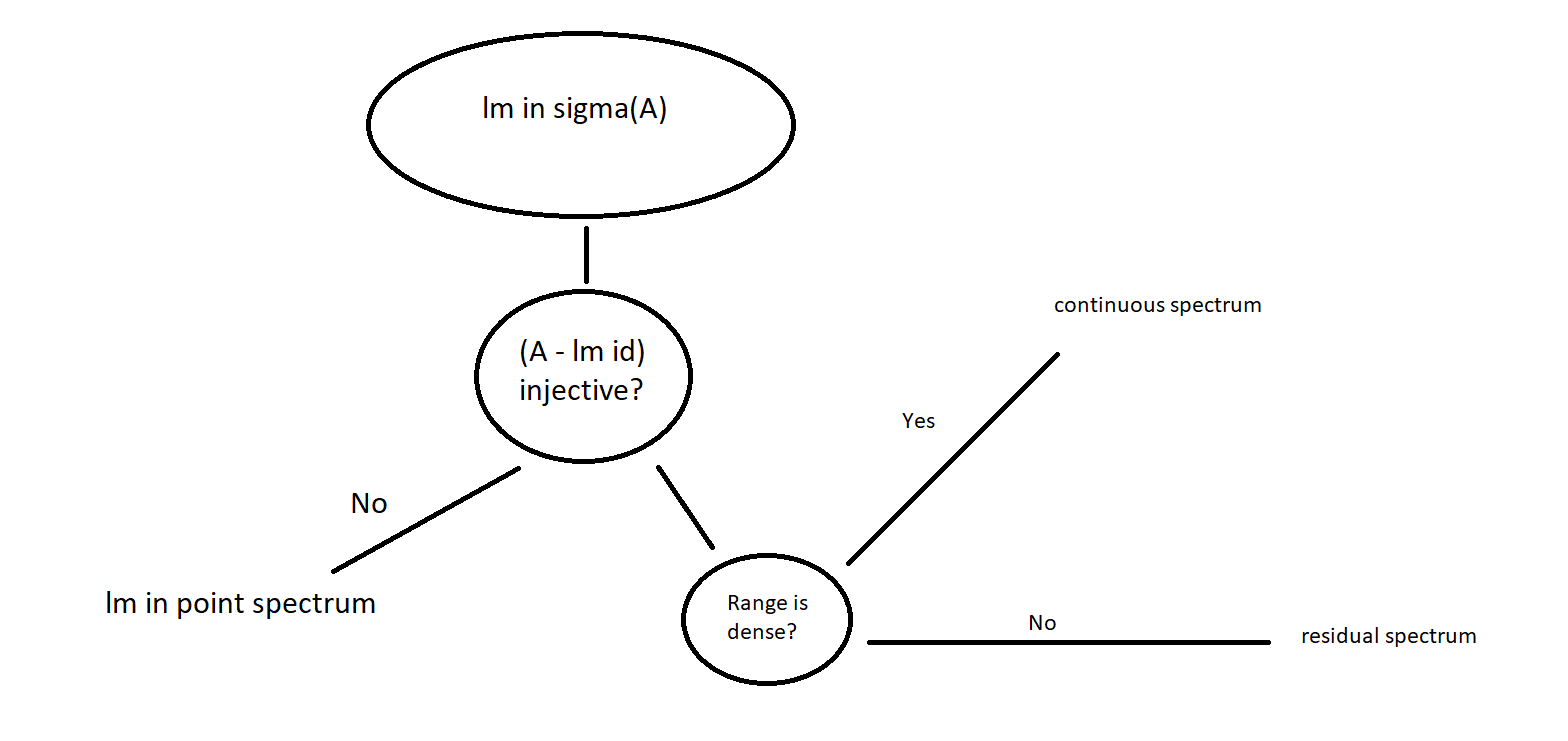
\includegraphics[width = 0.7\textwidth]{image.png}
    \end{figure}

    \item If A is a bounded linear operator on a Hilbert space, then its resolvent $R_\lm = (\lm\id - A)\inv$ is defined on the exterior disk $\{ \lm \in \C : \norm{A} < |\lm|\}$. 

    \item If A is a bounded linear operator, then the spectral radius of A, denoted by $r(A)$ is the radius of the smallest disk centered at zero that contains $\sigma(A)$. That is, $r(A) = \sup \{|\lm| : \lm \in \sigma(A)\}$. 

    \item If A is a bounded linear operator, then the spectral radius is given as 
    \[r(A) = \lim_{n \to \infty} \norm{A^n}^{1/n}.\]
    If $A$ is self adjoint, then $r(A) = \norm{A}$.

    \item The eigenvalues of a bounded, self-adjoint linear operator are real, and eigenvectors associated with different eigenvalues are orthogonal. 

    \item If $\lm$ belongs to the residual spectrum of $A$, then $\overline{\lm}$ is an eigenvalue of $A\star$. 

    \item If A is a bounded, self-adjoint operator on a Hilbert space, then the spectrum of A is real and contained in the interval $[-\norm{A}, \norm{A}]$.
    
    \item The residual spectrum of a bounded, self-adjoint operator is empty.

    \boxedquote{Spectral Theorem for compact, self-adjoint operators}
    {
    Let $A : \scH \to \scH$ be a compact, self-adjoint operator on a Hilbert space $\scH$. There is an orthonormal basis of $\scH$ consisting of eigenvectors of $A$. The nonzero eigenvalues of $A$ form a finite or countably infinite set $\{\lm_k\}$ or real numbers, and 
    \[A = \sum_k \lm_k P_k =    \sum_k \lm_k \ketbra{v_k}{v_k} \]
    where $P_k$ is the orthogonal projection onto the finite-dimensional subspace of eigenvectors with eigenvalue $\lm_k$. If the number of nonzero eigenvalues is countably finite, then the series converges to $A$ in the operator norm. 
    }

    \boxedquote{Theorem 9.17}{Let $E$ be a subset of an infinite-dimensional, separable Hilbert space $\scH$.
    \begin{itemize}
        \item[a)] If $E$ is precompact, then for every orthonormal set $\{e_n : n \in \N\}$ and $\ep > 0$, there is an N such that
        \[\sum_{n = N+1}^\infty |\braket{e_n}{x}|^2 < \ep \quad \text{ for all} x \in E.\]
        \item[b)] If $E$ is bounded, and there is an orthonormal basis $\{e_n\}$ of $\scH$ with the property that for every $\ep > 0$ there is an $N$ such that the above summation holds, then $E$ is precompact. 
    \end{itemize}
    }

    \boxedquote{Hilbert-Schmidt Operators}{A bounded linear operator $A$ on a separable Hilbert space $\scH$ is \textit{Hilbert-Schmidt} if there is an orthonormal basis $\{e_n : n \in \N\}$ such that 
    \[\sum_{n = 1}^\infty \norm{Ae_n}^2 < \infty\]
    }
    \item If $A$ is a Hilbert-schmidt operator, then
    \[\norm{A}_{HS}^2 = \sum_{n = 1}^\infty \norm{Ae_n}^2\]
    is called the Hilbert-schmidt norm of $A$.

    \item A Hilbert-Schmidt operator is compact.

    \item An operator with finite rank is compact. 

    \item The uniform limit of compact operators is compact. 

\newpage
    \mquote{Theorem 9.24}{A bounded linear operator on a Hilbert space is compact if and only if it maps weakly convergent sequences into strongly convergent sequences. }
\end{itemize}
\end{document}